\documentclass[11pt]{standalone}
\usepackage{amssymb}
\usepackage{amsmath}
\usepackage[no-math]{fontspec}
\usepackage{unicode-math}
\setmainfont{Libertinus Sans}
\setsansfont{Libertinus Sans}
\setmathfont{Libertinus Math}
\usepackage{pgf,xcolor}
\usepackage{tikz}
\usetikzlibrary{arrows.meta, backgrounds, calc}
\usepackage{pgfplots}
\pgfplotsset{compat=newest}
\usepackage{pifont}

\definecolor{my_darkgray}{HTML}{484949}
\definecolor{my_lightgray}{HTML}{F3F4F4}
\definecolor{my_darkblue}{HTML}{005A94}
\definecolor{my_lightblue}{HTML}{CCDEE9}
\definecolor{my_yellow}{HTML}{FFEC7F}
\definecolor{my_red}{HTML}{E60000}
\definecolor{my_orange}{HTML}{E87846}

\begin{document}
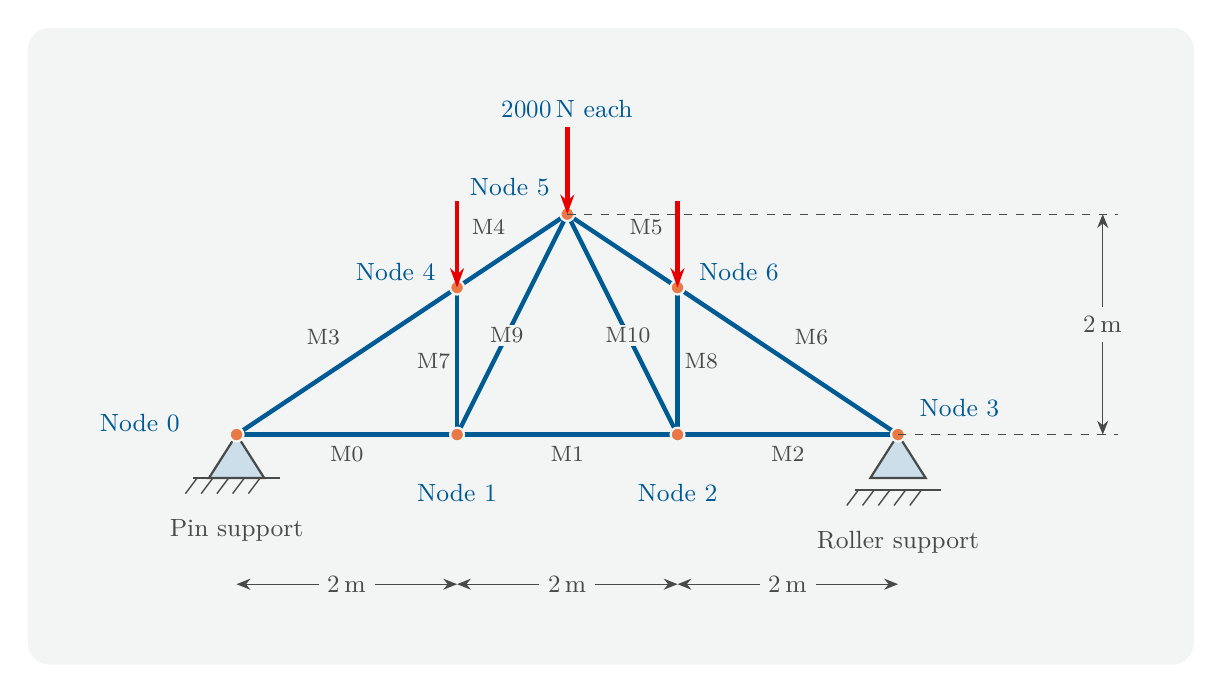
\begin{tikzpicture}[
    show background rectangle,
    background rectangle/.style={fill=my_lightgray, rounded corners=8pt},
    inner frame sep=0.8cm,
    annotation/.style={draw=my_darkgray, thick, -{Stealth[length=7pt, width=5pt]}},
    bemassung/.style={draw=my_darkgray, thin, {Stealth[length=5pt, width=4pt]}-{Stealth[length=5pt, width=4pt]}},
    stabnummer/.style={font=\footnotesize, text=my_darkgray, fill=my_lightgray, inner sep=1pt},
    last/.style={draw=my_red, ultra thick, -{Stealth[length=7pt, width=5pt]}}
]

    %------------------------------------------------------------
    % Knotenkoordinaten (Faktor 1.4 gegenüber Metern):
    % Knoten 0: (0,0), Knoten 1: (2,0), Knoten 2: (4,0), Knoten 3: (6,0),
    % Knoten 4: (2,4/3), Knoten 5: (3,2), Knoten 6: (4,4/3)
    %------------------------------------------------------------
    \coordinate (N0) at (0,0);
    \coordinate (N1) at (2.8,0);
    \coordinate (N2) at (5.6,0);
    \coordinate (N3) at (8.4,0);
    \coordinate (N4) at (2.8,1.8667);
    \coordinate (N5) at (4.2,2.8);
    \coordinate (N6) at (5.6,1.8667);

    %------------------------------------------------------------
    % Festlager an Knoten 0
    %------------------------------------------------------------
    \draw[fill=my_lightblue, draw=my_darkgray, thick]
        (N0) -- ++(-0.35,-0.55) -- ++(0.7,0) -- cycle;
    \draw[draw=my_darkgray, thick] ($(N0)+(-0.55,-0.55)$) -- ++(1.1,0);
    \foreach \x in {-0.5,-0.3,...,0.45} {
        \draw[draw=my_darkgray, line width=0.5pt] ($(N0)+(\x,-0.55)$) -- ++(-0.15,-0.2);
    }

    %------------------------------------------------------------
    % Loslager an Knoten 3 (Dreieck, Spalt, Rollenlinie)
    %------------------------------------------------------------
    \draw[fill=my_lightblue, draw=my_darkgray, thick]
        (N3) -- ++(-0.35,-0.55) -- ++(0.7,0) -- cycle;
    \draw[draw=my_darkgray, thick] ($(N3)+(-0.55,-0.7)$) -- ++(1.1,0);
    \foreach \x in {-0.5,-0.3,...,0.45} {
        \draw[draw=my_darkgray, line width=0.5pt] ($(N3)+(\x,-0.7)$) -- ++(-0.15,-0.2);
    }

    %------------------------------------------------------------
    % Stäbe (primäres Element): my_darkblue, ultra thick
    %------------------------------------------------------------
    \foreach \A/\B in {N0/N1, N1/N2, N2/N3, N0/N4, N4/N5, N5/N6, N6/N3,
                       N1/N4, N2/N6, N1/N5, N2/N5} {
        \draw[draw=my_darkblue, ultra thick] (\A) -- (\B);
    }

    %------------------------------------------------------------
    % Stabnummern in der Reihenfolge der Stabliste
    %------------------------------------------------------------
    \node[stabnummer] at ($(N0)!0.5!(N1)+(0,-0.25)$) {M0};
    \node[stabnummer] at ($(N1)!0.5!(N2)+(0,-0.25)$) {M1};
    \node[stabnummer] at ($(N2)!0.5!(N3)+(0,-0.25)$) {M2};
    \node[stabnummer] at ($(N0)!0.5!(N4)+(-0.3,0.3)$) {M3};
    \node[stabnummer] at ($(N4)!0.5!(N5)+(-0.3,0.3)$) {M4};
    \node[stabnummer] at ($(N5)!0.5!(N6)+(0.3,0.3)$) {M5};
    \node[stabnummer] at ($(N6)!0.5!(N3)+(0.3,0.3)$) {M6};
    \node[stabnummer] at ($(N1)!0.5!(N4)+(-0.3,0)$) {M7};
    \node[stabnummer] at ($(N2)!0.5!(N6)+(0.3,0)$) {M8};
    \node[stabnummer] at ($(N1)!0.45!(N5)$) {M9};
    \node[stabnummer] at ($(N2)!0.45!(N5)$) {M10};

    %------------------------------------------------------------
    % Knotenpunkte (hervorgehoben): my_orange, Rand my_lightgray
    %------------------------------------------------------------
    \foreach \P in {N0, N1, N2, N3, N4, N5, N6} {
        \draw[fill=my_orange, draw=my_lightgray, thick] (\P) circle (2.5pt);
    }

    %------------------------------------------------------------
    % Schneelast: 2000 N an den Knoten 4, 5 und 6
    %------------------------------------------------------------
    \foreach \P in {N4, N5, N6} {
        \draw[last] ($(\P)+(0,1.1)$) -- (\P);
    }
    \node[font=\small, text=my_darkblue, anchor=south] at ($(N5)+(0,1.1)$) {$2000\,\mathrm{N}$ each};

    %------------------------------------------------------------
    % Knotenbeschriftungen
    %------------------------------------------------------------
    \node[font=\small, text=my_darkblue, anchor=east]  at ($(N0)+(-0.6,0.15)$) {Node 0};
    \node[font=\small, text=my_darkblue, anchor=north] at ($(N1)+(0,-0.5)$) {Node 1};
    \node[font=\small, text=my_darkblue, anchor=north] at ($(N2)+(0,-0.5)$) {Node 2};
    \node[font=\small, text=my_darkblue, anchor=south west] at ($(N3)+(0.15,0.1)$) {Node 3};
    \node[font=\small, text=my_darkblue, anchor=east]  at ($(N4)+(-0.15,0.2)$) {Node 4};
    \node[font=\small, text=my_darkblue, anchor=south east] at ($(N5)+(-0.1,0.1)$) {Node 5};
    \node[font=\small, text=my_darkblue, anchor=west]  at ($(N6)+(0.15,0.2)$) {Node 6};

    %------------------------------------------------------------
    % Lagerbeschriftungen
    %------------------------------------------------------------
    \node[font=\small, text=my_darkgray, anchor=north] at ($(N0)+(0,-0.95)$) {Pin support};
    \node[font=\small, text=my_darkgray, anchor=north] at ($(N3)+(0,-1.1)$) {Roller support};

    %------------------------------------------------------------
    % Bemaßung
    %------------------------------------------------------------
    \draw[bemassung] (0,-1.9) -- node[font=\small, text=my_darkgray, fill=my_lightgray] {$2\,\mathrm{m}$} (2.8,-1.9);
    \draw[bemassung] (2.8,-1.9) -- node[font=\small, text=my_darkgray, fill=my_lightgray] {$2\,\mathrm{m}$} (5.6,-1.9);
    \draw[bemassung] (5.6,-1.9) -- node[font=\small, text=my_darkgray, fill=my_lightgray] {$2\,\mathrm{m}$} (8.4,-1.9);
    \draw[draw=my_darkgray, dashed, thin] (N5) -- (11.2,2.8);
    \draw[draw=my_darkgray, dashed, thin] (N3) -- (11.2,0);
    \draw[bemassung] (11,0) -- node[font=\small, text=my_darkgray, fill=my_lightgray] {$2\,\mathrm{m}$} (11,2.8);

\end{tikzpicture}
\end{document}
